%% This is an example first chapter.  You should put chapter/appendix that you
%% write into a separate file, and add a line \include{yourfilename} to
%% main.tex, where `yourfilename.tex' is the name of the chapter/appendix file.
%% You can process specific files by typing their names in at the 
%% \files=
%% prompt when you run the file main.tex through LaTeX.
\chapter{Introduction}
Some general introduction goes here. They will be added only after the thesis is finished. 
A brief description of what each chapter will be covering will also be covered in this section. 

\section{Introduction to q-TASEP}
\label{sec:intro-qtasep}

q-TASEP, short for q-deformed totally asymmetric simple exclusion process, refers to a continuous time, discrete space Markov Process $\vec{x}(t)$ describing the dynamics of the following interacting particle system:

\begin{itemize}
\item Particles denoted by $\{x_1, x_2, x_3, ...\}$ occupy sites of $\mathbb{Z}$ exclusively with positions at time $t$ denoted as $x_i(t)$. The particles are ordered in such a way that $x_i(t) < x_j(t)$ for $i > j$.
\item Particles jump to the right by one spot ($x_i(t)$ increases by $1$) with jump rate given by $a_i (1-q^{x_{i-1}(t)-x_i(t)+1})$ for $i \ge 2$, where $q \in [0,1)$, $a_i > 0$. The jump rate for the particle $x_1$ is defined to be $a_1$.
\item All jumps occur indenpendently of each other according to exponential clocks with parameter $1$.
\end{itemize}

\begin{figure}
	\centering
	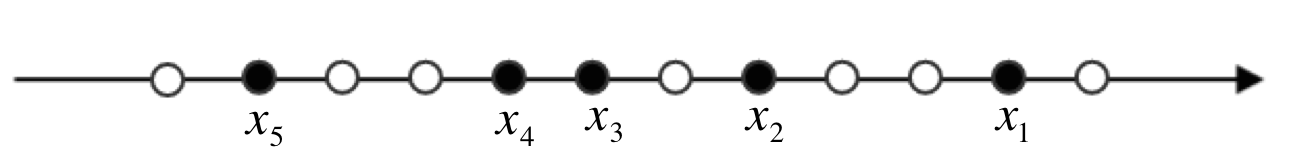
\includegraphics[width=0.5\textwidth]{q-TASEP}
	\caption[An illustration of q-TASEP]
	{An illustration of q-TASEP. The jump rate of the particle $x_2$ is given by $a_2(1-q^2)$, while that of the particle $x_4$ is $0$.}
	\label{fig:q-TASEP}
\end{figure}

It's worth noting that the ordering of the particles remains unchanged throughout the process. Note also that in the definition of q-TASEP, numbering of the particles starts with $1$. However, to facilitate our discussion, we could have added a virtual partical $x_0$ with $x_0 = \infty$ so that the jump rate of $x_1$ is also equal to $a_1 (1-q^{x_0(t) - x_1(t) + 1}) = a_1$. 

It can be easily seen that dynamics of the right most $N$ particles, i.e., particle $x_1$, $x_2$, $\dots$, $x_N$, is independent from those to the left of them, i.e., $x_{N+1}$, $x_{N+2}$, $\dots$ Therefore, from now onwards, we will be focusing on the study of q-TASEP with $N$ particles, with configuration $x_1(t) > x_2(t) > \dots > x_N(t)$. We could then define our state space as $$X^N = \{\vec{x}=(x_0,x_1,\dots, x_N) \in \{\infty \} \times \mathbb{Z}^N : \infty = x_0 > x_1 > \dots > x_N \}.$$

For q-TASEP with $N$ particles, the infinitesimal generator of $\vec{x}(t)$ acting on suitable function $f: X^N \rightarrow \mathbb{R}$, denoted by $L^{q-TASEP} f$, is given by $$(L^{q-TASEP} f) (\vec{x}) = \sum_{i=1}^{N} a_i (1-q^{x_{i-1} - x_i - 1}) (f(\vec{x}_i^{+}) - f(\vec{x})),$$ where $\vec{x}_i^{+}$ denotes the configuration of the q-TASEP with particle $x_i$ jumps to the right by $1$ position, i.e., $\vec{x}_i^+ = (x_0, x_1, \dots, x_{i-1}, x_i+1, x_{i+1}, \dots, x_N)$. This follows from the fact that for $t$ small, there is only $1$ chance for one of the $N$ particles to jump according its own jump rate.

\section{Initial data for q-TASEP}
For a q-TASEP to be well defined, additional to the dynamics of q-TASEP described in Section \ref{sec:intro-qtasep}, we also need an initial configuration of the process, called initial data. In this paper, we focus on two types of initial data, namely, the step initial data and the half stationary initial data. 

Step initial data is defined as the configuration of $x_i(0) = -i$ for $1 \le i \le N$. For half stationary initial data, we define q-Geometric distribution. 

\begin{definition}
\label{def:qgeo}
For $\alpha \in [0,1)$, we say that a random variable $X$ follows the q-Geometric distribution with parameter $\alpha$ [written as $X \sim qGeo(\alpha)$] if $$\mathbb{P}(X = k) = (\alpha;q)_{\infty} \frac{\alpha^k}{(q;q)_k},$$ where $(a;q)_n = (1-a)(1-aq)(1-aq^2)\dots(1-aq^{n-1})$ and $(a;q)_{\infty} = (1-a)(1-aq)(1-aq^2)\dots$
\end{definition}

Let $X_i \sim qGeo(\alpha/a_i)$ for $1 \le i \le N$ be $N$ independent q-Geometric random variables. Then the half stationary initial condition is defined recursively by first setting $x_1(0) = -1 + X_1$ and letting $x_i(0) = -1 + x_{i-1}(0) + X_i$ for $i > 1$. Note that when $\alpha = 0$, the step initial data is recovered.

\section{q-TASEP for a few particles}
The main goal for the study of q-TASEP in this thesis is to identify an exact formula for the distribution of the particle positions, $\mathbb{P}(x_N(t) = m)$ for $m \in \mathbb{Z}$ with step and half stationary initial data. In this section, we provide some intuitions of how this problem can be approached via elementary methods for q-TASEP of $1$ and $2$ particles, thereby illustrating how the complexity grows for $N$ large. 

\subsection{q-TASEP with $1$ particle}
In this section we focus on the q-TASEP with only $1$ particle denoted by $x_1$ starting at position $x_1(0) = 0$. Let $T_i$, $i = 1,2,\dots$ be independent and identically distributed exponential random variables with parameter $1$ denoting the time between the $(i-1)th$ and the $ith$ jump. For $m \in \mathbb{Z}_{\ge 0}$, define $$a_m = \mathbb{P}(x_1(t) \le m) = \mathbb{P}(\sum_{i=1}^{m+1} T_i > t)$$ such that $\mathbb{P}(x_1(t) = m) = a_m - a_{m-1}$ for $m \ge 1$ and $\mathbb{P}(x_1(t) = 0) = a_0 = e^{-t}$. Since $T_i \sim exp(1)$, $\sum_{i=1}^{m} T_i \sim Erlang(m,1)$ and therfore, by the density function of Erlang distribution, $$1 - a_m = \int_0^t \frac{s^m}{m!} e^{-s} ds.$$ 

\begin{proposition}
For q-TASEP with one particle $x_1$ with step initial condition, i.e., $x_1(0) = -1$, then $\mathbb{E}[x_1(t)+1] = t$ and $\mathbb{E}[q^{x_1(t)+1}] = e^{(q-1)t}$.
\end{proposition}

\begin{proof}
From the notations above, we have that $\mathbb{P}(x_1(t) = m) = a_m - a_{m-1}$, where $a_m$ is defined by $a_m = 1 - \int_0^t \frac{s^m}{m!} e^{-s} ds$. Therefore, we have
\begin{align}
\mathbb{E}[x_1(t)] &=  \lim_{n \to \infty} ((1-a_0) + (1-a_1) + ... + (1-a_{n-1}) - n ( 1-a_n))\\
  						&= \lim_{n \to \infty} (\int_{0}^{t} e^{-s}  (\sum_{i=0}^{n-1} \frac{s^i}{i!}) ds) +\lim_{n \to \infty} (n \times \int_{0}^{t} \frac{s^n}{n!} e^{-s} ds)\\
						&=  \int_{0}^{t} e^{-s} \lim_{n \to \infty} (\sum_{i=0}^{n-1} \frac{s^i}{i!}) ds + 0\\
						&=  \int_{0}^{t} e^{-s} e^s dt\\
						&= t
\end{align}
Moreover, $\mathbb{E}[q^{x_0(t)}]$ can be computed as below: 
\begin{align}
\mathbb{E}[q^{x_0(t)}] &= \lim_{n \to \infty} (q^0  a_0 + \sum_{i=1}^{n} q^i (a_i - a_{i-1}) )\\
											 &= \lim_{n \to \infty} (-(1-q) (\sum_{i=0}^{n-1} q^i (1-a_i)) - q^n (1-a_n) + 1)\\
											 &= - (1-q) \lim_{n \to \infty} ( \int_{0}^{t} e^{-s} \sum_{i=0}^{n-1} q^i \frac{s^i}{i!} ds) - \lim_{n \to \infty} \int_0^t q^n \frac{s^n}{n!} ds + 1\\
											 &=  - (1-q) \int_0^t e^{-s }  \lim_{n \to \infty} \sum_{i=0}^{n-1} q^i \frac{s^i}{i!} ds- \lim_{n \to \infty} \int_0^t q^n \frac{s^n}{n!} ds + 1\\
				     					 &=  - (1-q) \int_0^t e^{-s } e^{qs}  ds -\lim_{n \to \infty}  \int_0^t q^n \frac{s^n}{n!} ds + 1\\
				     					 &= e^{(q-1)t}.
\end{align}
\end{proof}

\subsection{q-TASEP with $2$ particles}
Situation starts to get more complicated when there are $2$ particles in the q-TASEP system. 

\section{Introduction to q-TAZRP}
Next, we introduce another Markov process called q-TAZRP, short for q-deformed totally asymmetric zero range process. q-TAZRP on an interval $\{0,1,...,N\}$ is a continuous time, discrete space Markov process $\vec{y}(t)$ with state space $$Y^N = (\mathbb{Z}_{\ge 0})^{N+1}$$ subject to the condition of $\sum_{i=0}^{N} y_i(t) = \sum_{i=0}^{N} y_i(0)$ $\forall$ $t\in\mathbb{R}_{\ge 0}$. Dynamics of a q-TAZRP is defined as the following:
\begin{itemize}
\item For each $i \in \{1,2,\dots,N\}$, $y_i(t)$ decreases by $1$ and $y_{i-1}(t)$ increases by $1$ simultaneously according to a rate function given by $g_i(k) = a_i (1-q^{y_i(t)})$.
\item All changes occur independently for each site according to exponential clocks.
\item $y_0$ is always non-decreasing.
\end{itemize}

\begin{figure}
	\centering
	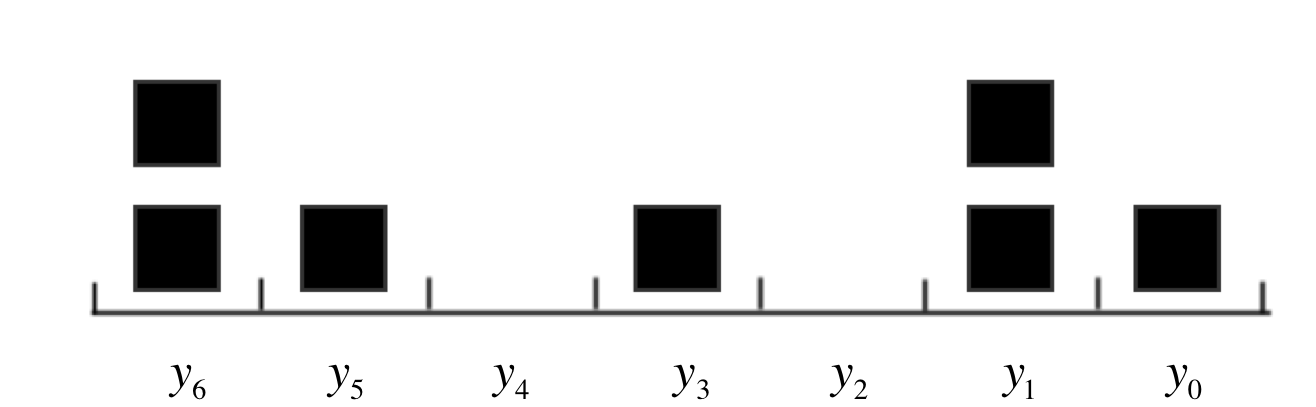
\includegraphics[width=0.75\textwidth]{q-TAZRP}
	\caption[An illustration of q-TAZRP]
	{An illustration of q-TAZRP. Rate function for site $y_1$ is given by $a_1 (1-q^2)$.}
	\label{fig:qTAZRP}
\end{figure}

A natural interpretation of the q-TAZRP is given in Figure \ref{fig:qTAZRP}, where a total of $\sum_{i=0}^{N} y_i(0)$ particles occupy the $N$ sites ordered in such a way that $y_i$ is to the left of $y_{i-1}$ for $i = 1,2,\dots,N$. The changes in the definition then refer to a jump of the top particle at site $y_i$ to the site $y_{i-1}$. Note then that no particle leaves site $0$.

It can be shown that the infinitesimal generator of $\vec{y}(t)$ acting on a suitable function $h:Y^N \rightarrow \mathbb{R}$, denoted as $L^{q-TAZRP} h$, is given by $$(L^{q-TAZRP} h)(\vec{y}) = \sum_{i=1}^{N} a_i (1-q^{y_i}) (h(\vec{y}^{i,i-1}) - h(\vec{y})),$$ where $\vec{y}^{i,i-1}$ represents the configuration of $(y_0, \dots, y_{i-2}, y_{i-1}+1, y_i - 1, y_{i+1}, \dots, y_N)$.